\chapter{Wstęp i cel pracy}


\noindent Od wielu lat robotyka prężnie się rozwija czego dowodem jest wzrost liczby publikacji dotyczących zagadnień ...

W robotyce można wyróżnić kilka podstawowych typów manipulatorów


Lorem ipsum dolor sit amet, consectetur adipiscing elit, sed do eiusmod tempor incididunt ut labore et dolore magna aliqua. Ut enim ad minim veniam, quis \textcolor{red}{nostrud exercitation $x=5y$ ullamco laboris nisi ut aliquip ex ea commodo consequat.} Duis aute irure dolor in reprehenderit in voluptate velit $$x=5y$$ esse cillum dolore eu fugiat nulla pariatur. \sout{\textbf{Excepteur sint occaecat cupidatat non proident, sunt in culpa} qui officia deserunt mollit anim id est laborum.}
\begin{equation}
\label{eq:prawo_newtona}
a = \geq \frac{F}{m}   
\end{equation}
Równanie nienumerowane
\begin{equation*}
\label{eq:prawo_newtona2}
\int\limits_{-\infty}^{6x+83^5} a_3^4 da_3 = \left( \frac{\mathbf{F}}{\sqrt{m^2}}    \right) \in \mathcal{C} \to \infty \begin{bmatrix}a   & b \\ c   & d  \end{bmatrix} \quad \qquad \text{for all $x$}
\end{equation*}


\noindent \textbf{Lista punktowana}

\begin{itemize}
    \item Punkt 1
    \item Punkt 2
    \begin{itemize}
        \item Podpunkt 2.1
        \item Podpunkt 2.2
        \begin{itemize}
            \item Podpunkt 2.2.1
            \item Podpunkt 2.2.2
        \end{itemize}
    \end{itemize}
    \item Punkt 3
\end{itemize}

\noindent \textbf{Lista numerowana}

\begin{enumerate}
    \item Punkt 1
    \item Punkt 2
    \begin{enumerate}
        \item Podpunkt 2.1
        \item Podpunkt 2.2
        \begin{itemize}
            \item Podpunkt 2.2.1
            \item Podpunkt 2.2.2
        \end{itemize}
    \end{enumerate}
    \item Punkt 3
\end{enumerate}

\section{Wstęp teoretyczny}

Podstawowym równaniem w teorii obwodów jest prawo Ohma dane następującym wzorem \cite{Now02}:

\begin{equation}
\label{eq:prawo_ohma}
U = I R    
\end{equation}
gdzie $U$ oznacza napięcie [\si{\volt}], $R$ oznacza rezystancję [\si{\ohm}], natomiast $I$ oznacza natężenie prądu [\si{\ampere}], patrz \cref{tab:nasza_tabela}. Kod pokazuje \cref{lst:kod}

\color{blue}
\subsection{Algorytmy szukania ścieżek}

\subsubsection{Algorytm A*}

co zostało uwzględnione w \cref{eq:prawo_ohma}, oraz użyte w \cite{Nat12,Bar04}

\subsubsection{Złożoność obliczeniowa} 

\begin{figure}[h]
    \centering
    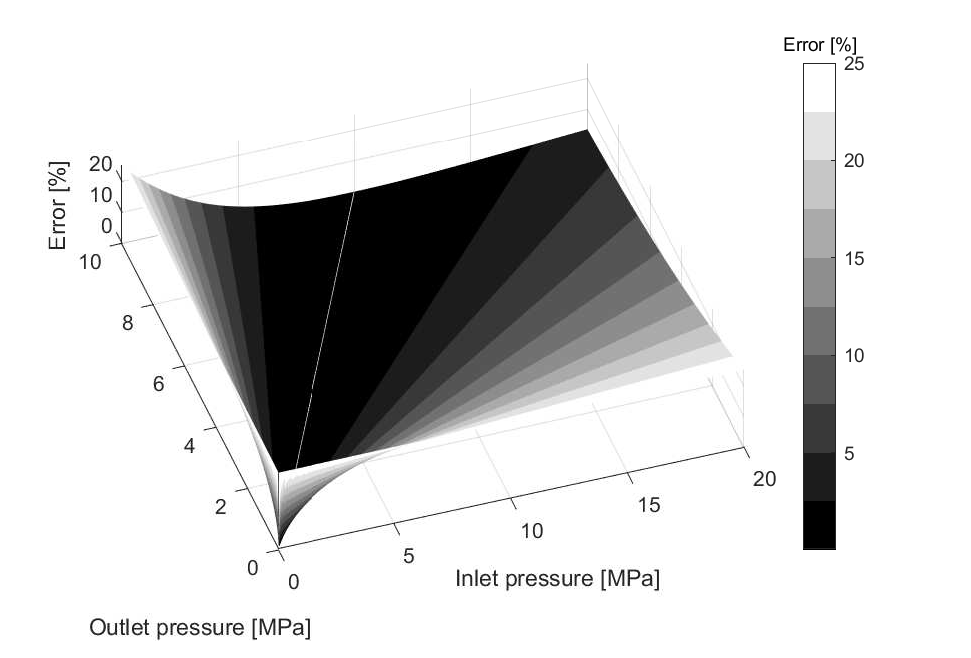
\includegraphics[width=0.7\textwidth]{./img/Figure3.eps}
    \caption{Zależność błędu od czegoś innego asf sdf sdf sdffksd k lkhjfkjsd sdf dfss o ooo  dsfsdf fdsf sdfffff sdf sssss dsfsdff sdf}
    \label{fig:nasz_obrazek}
\end{figure}

\section{Cel pracy}

Co widać na \cref{fig:nasz_obrazek}. \Cref{fig:nasz_obrazek} prezentuje

\begin{table}[b]%t - top, h - here, b - bottom
    \centering
    \caption{Podpis tabeli}
    \begin{tabular}{|c|c||}
        \hline
        \textbf{Nagłówek 1} & \textbf{Nagłówek 2 } \\ \hline
        4 & 89  \\ \hline
    \end{tabular}
    \label{tab:nasza_tabela}
\end{table}
\section{Układ pracy}

\cref{chap:przeglad} zawiera przegląd literatury, wyszczególniając ...

\begin{lstlisting}[language=Python,caption={Opis kodu},captionpos=b,label={lst:kod}]
import numpy as np
    
def incmatrix(genl1,genl2):
    m = len(genl1)
    n = len(genl2)
    M = None #to become the incidence matrix
    VT = np.zeros((n*m,1), int)  #dummy variable
    
    return M
\end{lstlisting}


\begin{figure}
    \centering
    \begin{subfigure}[b]{0.48\textwidth}
        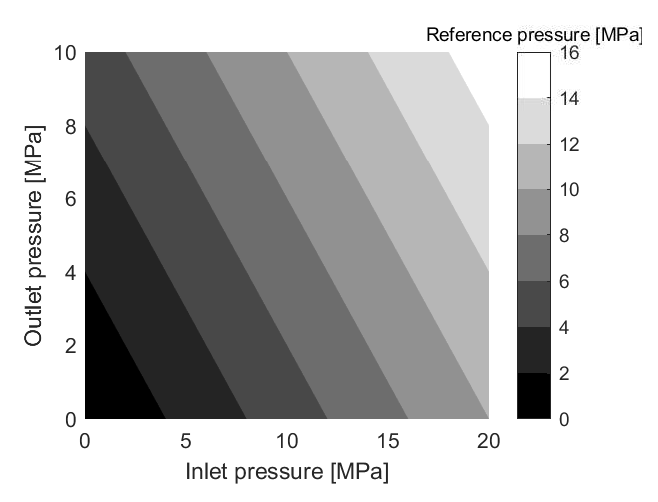
\includegraphics[width=\textwidth]{img/Figure1a.eps}
        \caption{Arithmetic mean approach (DW).}
        \label{fig:refpresdw}
    \end{subfigure}
    \begin{subfigure}[b]{0.48\textwidth}
        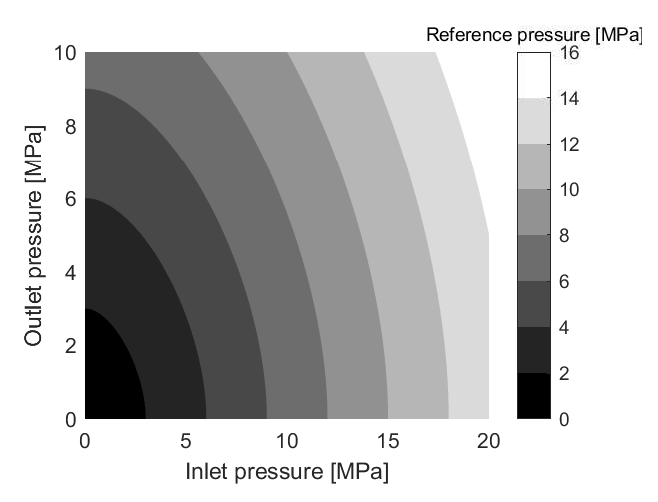
\includegraphics[width=\textwidth]{img/Figure1b.eps}
        \caption{Integral mean approach (PM).}
        \label{fig:refprespm}
    \end{subfigure}
    \begin{subfigure}[b]{0.48\textwidth}
        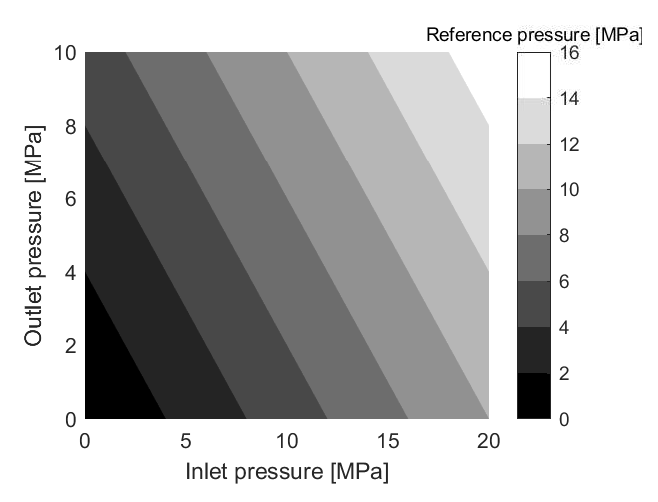
\includegraphics[width=\textwidth]{img/Figure1a.eps}
        \caption{Arithmetic mean approach (DW).}
        \label{fig:refpresdw2}
    \end{subfigure}
    \begin{subfigure}[b]{0.48\textwidth}
        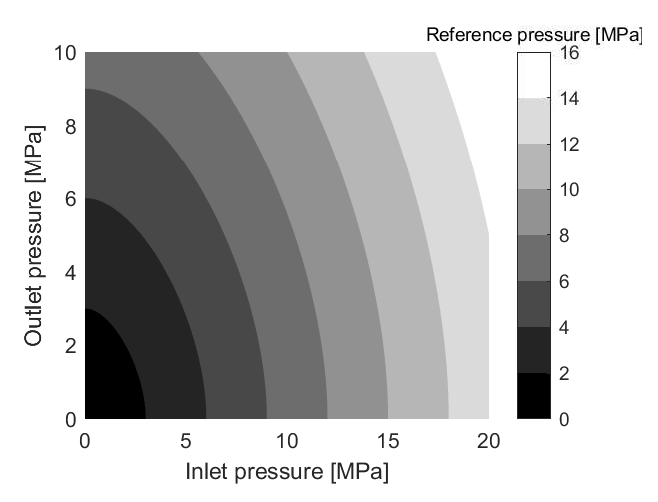
\includegraphics[width=\textwidth]{img/Figure1b.eps}
        \caption{Integral mean approach (PM).}
        \label{fig:refprespm2}
    \end{subfigure}
    \caption{Reference pressure calculated as the arithmetic mean (a) and the integral mean (b) over the pressure plane $\mathbf{p}$.}\label{fig:refpres}
\end{figure}